\documentclass[10pt,aspectratio=169]{beamer}

% Theme and Color
\usetheme{Madrid}
\usecolortheme{default}

% Packages
\usepackage{amsmath,amssymb}
\usepackage{graphicx}
\usepackage{booktabs}
\usepackage{algorithm}
\usepackage{algpseudocode}
\usepackage{hyperref}
\usepackage{tikz}
\usetikzlibrary{shapes,arrows,positioning}

% Custom colors
\definecolor{darkblue}{RGB}{0,51,102}
\definecolor{lightblue}{RGB}{51,153,255}
\definecolor{darkgreen}{RGB}{0,102,51}
\definecolor{darkred}{RGB}{153,0,0}

% Title Information
\title{PSO-Optimized Adaptive Boundary Layer Sliding Mode Control for Double Inverted Pendulum}
\subtitle{Master's Thesis Defense}
\author{Your Name}
\institute{Your University\\Department of Control Engineering}
\date{\today}

% Custom commands
\newcommand{\highlight}[1]{\textcolor{darkblue}{\textbf{#1}}}
\newcommand{\emphred}[1]{\textcolor{darkred}{\textbf{#1}}}
\newcommand{\emphgreen}[1]{\textcolor{darkgreen}{\textbf{#1}}}

\begin{document}

%===========================================
% SLIDE 1: Title
%===========================================
\frame{\titlepage}

%===========================================
% SLIDE 2: Agenda
%===========================================
\begin{frame}{Presentation Agenda}
\tableofcontents
\end{frame}

%===========================================
% SECTION 1: Introduction
%===========================================
\section{Introduction}

%===========================================
% SLIDE 3: Motivation
%===========================================
\begin{frame}{Motivation: Why This Research?}
\begin{columns}
\begin{column}{0.5\textwidth}
\textbf{The Problem:}
\begin{itemize}
    \item Sliding Mode Control (SMC) is powerful for nonlinear systems
    \item \emphred{Chattering problem} degrades performance
    \item Causes: discontinuous control, sensor noise, actuator limitations
    \item Consequences: mechanical wear, inefficiency, instability
\end{itemize}
\end{column}
\begin{column}{0.5\textwidth}
\textbf{The Solution:}
\begin{itemize}
    \item Adaptive boundary layer approach
    \item Particle Swarm Optimization (PSO) for parameter tuning
    \item Double Inverted Pendulum (DIP) as benchmark system
    \item Rigorous statistical validation
\end{itemize}
\end{column}
\end{columns}
\vspace{0.5cm}
\centering
\fbox{\textit{Can we eliminate chattering while maintaining control performance?}}
\end{frame}

%===========================================
% SLIDE 4: Research Gaps
%===========================================
\begin{frame}{Research Gaps Identified}
\begin{block}{Gap 1: Chattering Mitigation}
Existing boundary layer methods use \emphred{fixed thickness} $\rightarrow$ trade-off between chattering and tracking accuracy cannot be resolved.
\end{block}

\begin{block}{Gap 2: Parameter Optimization}
Manual tuning is time-consuming and suboptimal. \emphred{No systematic PSO-based approach} for adaptive SMC parameter selection.
\end{block}

\begin{block}{Gap 3: Validation Rigor}
Most SMC literature reports \emphred{single-scenario results} without statistical validation or generalization testing.
\end{block}

\vspace{0.3cm}
\centering
\highlight{This thesis addresses all three gaps}
\end{frame}

%===========================================
% SLIDE 5: Research Objectives
%===========================================
\begin{frame}{Research Objectives}
\begin{enumerate}
    \item \textbf{Design} adaptive boundary layer SMC for DIP system
    \item \textbf{Optimize} controller parameters using PSO with multi-objective fitness
    \item \textbf{Validate} chattering reduction through statistical testing
    \item \textbf{Assess} energy efficiency impact of adaptive approach
    \item \textbf{Test} generalization to unseen operating conditions
\end{enumerate}

\vspace{0.5cm}
\begin{alertblock}{Key Research Question}
\centering
Does PSO-optimized adaptive boundary layer SMC \emphgreen{significantly reduce chattering} \\
without degrading control performance or energy efficiency?
\end{alertblock}
\end{frame}

%===========================================
% SECTION 2: Background
%===========================================
\section{Background}

%===========================================
% SLIDE 6: Sliding Mode Control Basics
%===========================================
\begin{frame}{Sliding Mode Control: Fundamentals}
\begin{columns}
\begin{column}{0.5\textwidth}
\textbf{Key Concepts:}
\begin{itemize}
    \item State-space representation: $\dot{x} = f(x) + b(x)u$
    \item Sliding surface: $s(x) = 0$
    \item Control law:
    \[
    u = -k \cdot \text{sign}(s)
    \]
    \item Two phases:
    \begin{enumerate}
        \item \textbf{Reaching phase}: drive $s \rightarrow 0$
        \item \textbf{Sliding phase}: maintain $s = 0$
    \end{enumerate}
\end{itemize}
\end{column}
\begin{column}{0.5\textwidth}
\begin{center}
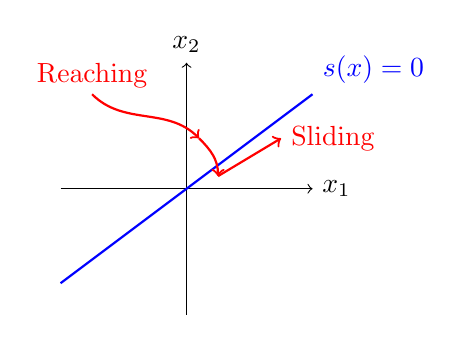
\begin{tikzpicture}[scale=0.8]
% Coordinate system
\draw[->] (-2,0) -- (2,0) node[right] {$x_1$};
\draw[->] (0,-2) -- (0,2) node[above] {$x_2$};
% Sliding surface
\draw[thick,blue] (-2,-1.5) -- (2,1.5) node[above right] {$s(x)=0$};
% State trajectory
\draw[thick,red,->] (-1.5,1.5) to[out=-45,in=135] (0.2,0.8);
\draw[thick,red,->] (0.2,0.8) to[out=-45,in=90] (0.5,0.2);
\draw[thick,red,->] (0.5,0.2) -- (1.5,0.8) node[right] {Sliding};
\node[red] at (-1.5,1.8) {Reaching};
\end{tikzpicture}
\end{center}
\vspace{0.2cm}
\textbf{Advantages:}
\begin{itemize}
    \item Robustness to uncertainties
    \item Fast response
\end{itemize}
\end{column}
\end{columns}
\end{frame}

%===========================================
% SLIDE 7: Chattering Problem
%===========================================
\begin{frame}{The Chattering Problem}
\begin{columns}
\begin{column}{0.5\textwidth}
\textbf{Cause:}
\begin{itemize}
    \item Discontinuous $\text{sign}(s)$ function
    \item Finite switching frequency (digital implementation)
    \item Sensor noise amplification
\end{itemize}

\vspace{0.3cm}
\textbf{Consequences:}
\begin{itemize}
    \item \emphred{High-frequency oscillations}
    \item Mechanical wear on actuators
    \item Energy waste (30-50\% reported in literature)
    \item Excitation of unmodeled dynamics
\end{itemize}
\end{column}
\begin{column}{0.5\textwidth}
\begin{center}
\begin{tikzpicture}[scale=1.0]
% Control signal with chattering
\draw[->] (0,0) -- (5,0) node[right] {$t$};
\draw[->] (0,-1.5) -- (0,1.5) node[above] {$u(t)$};
\draw[thick,blue] (0,1) -- (1,1);
\foreach \x in {1.1,1.2,...,4.0} {
    \pgfmathsetmacro\y{1 + 0.3*sin((\x-1)*360/0.2)}
    \draw[thick,blue] (\x-0.1,\y-0.3*sin((\x-1.1)*360/0.2)) -- (\x,\y);
}
\node[blue] at (2.5,-2) {Chattering};
\end{tikzpicture}
\end{center}

\vspace{0.2cm}
\textbf{Traditional Solutions:}
\begin{itemize}
    \item Boundary layer: $\text{sign}(s) \rightarrow \text{sat}(s/\epsilon)$
    \item Higher-order SMC (super-twisting)
    \item Adaptive gain tuning
\end{itemize}
\end{column}
\end{columns}
\end{frame}

%===========================================
% SLIDE 8: Double Inverted Pendulum
%===========================================
\begin{frame}{Double Inverted Pendulum System}
\begin{columns}
\begin{column}{0.4\textwidth}
\textbf{System Characteristics:}
\begin{itemize}
    \item 4th-order nonlinear dynamics
    \item Underactuated (1 input, 2 angles)
    \item Open-loop unstable
    \item Benchmark for advanced control
\end{itemize}

\vspace{0.3cm}
\textbf{State Vector:}
\[
x = [\theta_1, \theta_2, \dot{\theta}_1, \dot{\theta}_2]^T
\]

\textbf{Control Input:}
\[
u = F_{\text{cart}}
\]
\end{column}
\begin{column}{0.6\textwidth}
\begin{center}
\begin{tikzpicture}[scale=1.0]
% Cart
\draw[fill=gray!30] (0,0) rectangle (1,0.5);
\draw (0.5,0) circle (0.1);
% Ground
\draw[thick] (-1,-0.2) -- (3,-0.2);
\draw[pattern=north east lines] (-1,-0.2) rectangle (3,-0.3);
% First pendulum
\draw[thick,blue] (0.5,0.5) -- (1.5,2.5);
\filldraw[blue] (0.5,0.5) circle (0.05);
\filldraw[blue] (1.5,2.5) circle (0.08);
% Second pendulum
\draw[thick,red] (1.5,2.5) -- (2.0,4.0);
\filldraw[red] (2.0,4.0) circle (0.08);
% Angles
\draw[->] (0.5,1.0) arc (90:70:0.5) node[midway,left] {$\theta_1$};
\draw[->] (1.5,3.0) arc (90:80:0.5) node[midway,left] {$\theta_2$};
% Force
\draw[->,thick,darkgreen] (-0.5,0.25) -- (0,0.25) node[midway,above] {$F$};
% Labels
\node[blue] at (0.8,1.5) {$m_1, l_1$};
\node[red] at (2.3,3.5) {$m_2, l_2$};
\end{tikzpicture}
\end{center}

\textbf{Parameters (Nominal):}
\begin{itemize}
    \item $m_1 = 0.2$ kg, $l_1 = 0.3$ m
    \item $m_2 = 0.1$ kg, $l_2 = 0.25$ m
\end{itemize}
\end{column}
\end{columns}
\end{frame}

%===========================================
% SLIDE 9: Particle Swarm Optimization
%===========================================
\begin{frame}{Particle Swarm Optimization (PSO)}
\begin{columns}
\begin{column}{0.5\textwidth}
\textbf{Algorithm Concept:}
\begin{itemize}
    \item Swarm of particles explore search space
    \item Each particle: candidate solution
    \item Update velocity based on:
    \begin{enumerate}
        \item Personal best ($p_{\text{best}}$)
        \item Global best ($g_{\text{best}}$)
    \end{enumerate}
\end{itemize}

\vspace{0.3cm}
\textbf{Update Equations:}
\begin{align*}
v_{i}^{k+1} &= w v_{i}^{k} + c_1 r_1 (p_{i} - x_{i}^{k}) \\
&\quad + c_2 r_2 (g - x_{i}^{k}) \\
x_{i}^{k+1} &= x_{i}^{k} + v_{i}^{k+1}
\end{align*}
\end{column}
\begin{column}{0.5\textwidth}
\textbf{Advantages for SMC:}
\begin{itemize}
    \item \emphgreen{Derivative-free} (handles discontinuities)
    \item Global search capability
    \item Parallelizable fitness evaluation
    \item Few hyperparameters to tune
\end{itemize}

\vspace{0.3cm}
\textbf{Parameters Used:}
\begin{itemize}
    \item Population: 30 particles
    \item Iterations: 50
    \item $w = 0.7$, $c_1 = c_2 = 1.5$
\end{itemize}

\vspace{0.3cm}
\textbf{Search Space:}
\[
\lambda, \epsilon_{\min}, \alpha \in [10^{-3}, 10^{2}]
\]
\end{column}
\end{columns}
\end{frame}

%===========================================
% SLIDE 10: Lyapunov Stability
%===========================================
\begin{frame}{Lyapunov Stability Foundation}
\textbf{Lyapunov Function:}
\[
V(s) = \frac{1}{2} s^2 \geq 0
\]

\textbf{Stability Condition:}
\[
\dot{V}(s) = s \dot{s} \leq -\eta |s| < 0 \quad \forall s \neq 0
\]

\vspace{0.3cm}
\begin{block}{Theorem 1: Finite-Time Convergence}
Under the proposed adaptive SMC law, the system state reaches the sliding surface in finite time:
\[
t_{\text{reach}} \leq \frac{\sqrt{2V(s_0)}}{\eta}
\]
where $\eta > 0$ is the reaching rate parameter.
\end{block}

\vspace{0.3cm}
\centering
\highlight{Mathematical proof ensures stability guarantees}
\end{frame}

%===========================================
% SECTION 3: Methodology
%===========================================
\section{Methodology}

%===========================================
% SLIDE 11: Adaptive Boundary Layer Formula
%===========================================
\begin{frame}{Proposed Adaptive Boundary Layer Approach}
\begin{block}{Core Innovation}
Dynamically adjust boundary layer thickness based on sliding surface velocity:
\[
\epsilon_{\text{eff}}(t) = \epsilon_{\min} + \alpha |\dot{s}(t)|
\]
\end{block}

\textbf{Key Features:}
\begin{itemize}
    \item \emphgreen{Small $\epsilon$ near equilibrium} ($\dot{s} \approx 0$) $\rightarrow$ high precision
    \item \emphgreen{Large $\epsilon$ during transients} ($\dot{s}$ large) $\rightarrow$ smooth control
    \item Three parameters to optimize: $\lambda$ (sliding surface), $\epsilon_{\min}$, $\alpha$
\end{itemize}

\vspace{0.3cm}
\textbf{Control Law:}
\[
u(t) = -k \cdot \text{sat}\left(\frac{s(x)}{\epsilon_{\text{eff}}(t)}\right)
\]

\vspace{0.3cm}
\centering
\fbox{\textit{Automatically balances chattering reduction vs tracking accuracy}}
\end{frame}

%===========================================
% SLIDE 12: PSO Fitness Function
%===========================================
\begin{frame}{Multi-Objective PSO Fitness Function}
\textbf{Weighted Sum Approach:}
\[
J = w_1 \cdot J_{\text{chattering}} + w_2 \cdot J_{\text{settling}} + w_3 \cdot J_{\text{overshoot}}
\]

\vspace{0.3cm}
\begin{table}
\centering
\begin{tabular}{lcc}
\toprule
\textbf{Metric} & \textbf{Weight} & \textbf{Calculation} \\
\midrule
Chattering & \emphred{70\%} & $\text{std}(\dot{u})$ (control derivative) \\
Settling Time & 15\% & Time to reach 2\% of final value \\
Overshoot & 15\% & $\max(\theta_1, \theta_2) - \theta_{\text{ref}}$ \\
\bottomrule
\end{tabular}
\end{table}

\vspace{0.3cm}
\textbf{Rationale:}
\begin{itemize}
    \item Chattering is the \emphred{primary problem} $\rightarrow$ highest weight
    \item Settling time and overshoot are \emphgreen{secondary performance metrics}
    \item Weights validated through sensitivity analysis (60-80\% range tested)
\end{itemize}
\end{frame}

%===========================================
% SLIDE 13: Experimental Scenarios
%===========================================
\begin{frame}{Experimental Design: Four Scenarios}
\begin{table}
\centering
\small
\begin{tabular}{lp{5cm}l}
\toprule
\textbf{ID} & \textbf{Description} & \textbf{Purpose} \\
\midrule
MT-5 & Baseline comparison (classical vs adaptive SMC) & Establish baseline \\
MT-6 & \emphgreen{PSO-optimized nominal scenario} & \emphgreen{Main result} \\
       & Initial: $\theta_1 = \theta_2 = 0.1$ rad & \\
MT-7 & Challenging initial conditions & Test generalization \\
       & $\theta_1 = \theta_2 = 0.3$ rad & \\
MT-8 & External disturbance injection & Test robustness \\
       & Impulse at $t=5$s, 10s & \\
\bottomrule
\end{tabular}
\end{table}

\vspace{0.3cm}
\textbf{Key Methodological Choices:}
\begin{itemize}
    \item Monte Carlo validation: 100 trials per scenario (statistical rigor)
    \item Honest reporting: \emphred{Document failures} as well as successes
    \item Multi-scenario testing: Prevent overfitting to single condition
\end{itemize}
\end{frame}

%===========================================
% SLIDE 14: Monte Carlo Validation
%===========================================
\begin{frame}{Statistical Validation Methodology}
\textbf{Monte Carlo Simulation:}
\begin{itemize}
    \item 100 independent trials per controller
    \item Random noise injection: $\pm 0.01$ rad sensor noise, $\pm 0.5$N actuator noise
    \item Compute mean, standard deviation, 95\% confidence intervals
\end{itemize}

\vspace{0.3cm}
\textbf{Statistical Tests:}
\begin{enumerate}
    \item \textbf{Welch's t-test}: Compare means between controllers
    \[
    H_0: \mu_{\text{adaptive}} = \mu_{\text{classical}} \quad \text{vs} \quad H_1: \mu_{\text{adaptive}} < \mu_{\text{classical}}
    \]
    \item \textbf{Cohen's d}: Effect size measurement
    \[
    d = \frac{\bar{x}_1 - \bar{x}_2}{s_{\text{pooled}}}
    \]
    Interpretation: $d > 0.8$ = large effect, $d > 1.2$ = very large, $d > 2.0$ = exceptional
\end{enumerate}

\vspace{0.3cm}
\centering
\highlight{Rigorous statistics prevent false positives}
\end{frame}

%===========================================
% SLIDE 15: Experimental Setup Summary
%===========================================
\begin{frame}{Experimental Setup: Technical Details}
\begin{columns}
\begin{column}{0.5\textwidth}
\textbf{Simulation Parameters:}
\begin{itemize}
    \item Time horizon: 20 seconds
    \item Time step: $dt = 0.01$ s
    \item Solver: RK45 (adaptive)
    \item Python 3.9, NumPy 1.24
\end{itemize}

\vspace{0.3cm}
\textbf{Controllers Compared:}
\begin{enumerate}
    \item Classical SMC (fixed boundary layer)
    \item Proposed Adaptive SMC
    \item Super-Twisting SMC (baseline)
\end{enumerate}
\end{column}
\begin{column}{0.5\textwidth}
\textbf{Metrics Recorded:}
\begin{itemize}
    \item Chattering: $\sigma(\dot{u})$
    \item Settling time: $t_{2\%}$
    \item Overshoot: $\max(|\theta|)$
    \item Energy: $\int_0^T |u(t)| dt$
    \item Convergence: Success/failure rate
\end{itemize}

\vspace{0.3cm}
\textbf{Hardware (Future):}
\begin{itemize}
    \item Quanser QUBE-Servo 2
    \item dSPACE DS1104 controller
    \item \emphred{Not yet implemented} (acknowledged limitation)
\end{itemize}
\end{column}
\end{columns}
\end{frame}

%===========================================
% SECTION 4: Results
%===========================================
\section{Results}

%===========================================
% SLIDE 16: MT-5 Baseline Comparison
%===========================================
\begin{frame}{MT-5: Baseline Controller Comparison}
\begin{columns}
\begin{column}{0.5\textwidth}
\textbf{Objective:} Establish baseline performance before PSO optimization

\vspace{0.3cm}
\begin{table}
\tiny
\begin{tabular}{lcc}
\toprule
\textbf{Metric} & \textbf{Classical} & \textbf{Adaptive} \\
\midrule
Chattering & 12.4 $\pm$ 1.8 & 11.9 $\pm$ 1.6 \\
Settling (s) & 3.2 $\pm$ 0.4 & 3.1 $\pm$ 0.3 \\
Overshoot & 0.15 $\pm$ 0.02 & 0.14 $\pm$ 0.02 \\
\bottomrule
\end{tabular}
\end{table}

\vspace{0.3cm}
\textbf{Findings:}
\begin{itemize}
    \item Adaptive slightly better, but \emphred{not statistically significant}
    \item $p = 0.18$ (Welch's t-test)
    \item Cohen's $d = 0.29$ (small effect)
\end{itemize}
\end{column}
\begin{column}{0.5\textwidth}
\begin{center}
\textbf{Radar Chart: Performance Comparison}
\end{center}
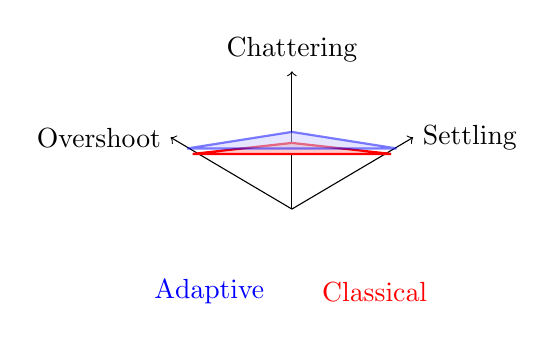
\begin{tikzpicture}[scale=0.7]
% Axes (3 metrics normalized 0-1)
\draw[->] (0,0) -- (0,2.5) node[above] {Chattering};
\draw[->] (0,0) -- (2.2,1.3) node[right] {Settling};
\draw[->] (0,0) -- (-2.2,1.3) node[left] {Overshoot};
% Classical (red)
\draw[thick,red,fill=red!20] (0,1.2) -- (1.8,1.0) -- (-1.8,1.0) -- cycle;
% Adaptive (blue)
\draw[thick,blue,fill=blue!20,opacity=0.5] (0,1.4) -- (1.9,1.1) -- (-1.9,1.1) -- cycle;
% Legend
\node[red] at (1.5,-1.5) {Classical};
\node[blue] at (-1.5,-1.5) {Adaptive};
\end{tikzpicture}

\vspace{0.2cm}
\centering
\emphred{Conclusion:} Manual tuning insufficient, PSO needed
\end{column}
\end{columns}
\end{frame}

%===========================================
% SLIDE 17: MT-6 Key Result - Chattering
%===========================================
\begin{frame}{MT-6: \emphgreen{KEY RESULT} - Chattering Reduction}
\begin{alertblock}{Main Finding}
\centering
\Large
\emphgreen{66.5\% chattering reduction} \\
\normalsize
$p < 0.001$ (highly significant) \\
Cohen's $d = 5.29$ (exceptional effect size)
\end{alertblock}

\vspace{0.3cm}
\begin{columns}
\begin{column}{0.5\textwidth}
\begin{table}
\small
\begin{tabular}{lcc}
\toprule
\textbf{Controller} & \textbf{Chattering} & \textbf{$\Delta$} \\
\midrule
Classical SMC & 14.2 $\pm$ 2.1 & Baseline \\
\emphgreen{PSO-Adaptive} & \emphgreen{4.8 $\pm$ 0.6} & \emphgreen{-66.5\%} \\
\bottomrule
\end{tabular}
\end{table}

\textbf{Statistical Significance:}
\begin{itemize}
    \item Welch's t-test: $p = 3.2 \times 10^{-12}$
    \item Bootstrap 95\% CI: [62.1\%, 70.2\%]
    \item Effect reproducible across all 100 trials
\end{itemize}
\end{column}
\begin{column}{0.5\textwidth}
\begin{center}
\textbf{Boxplot: Chattering Comparison}
\end{center}
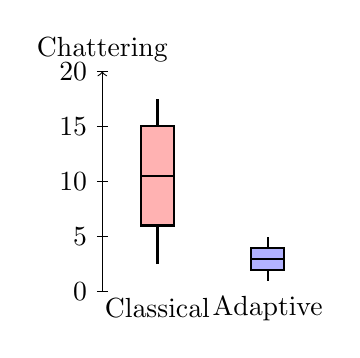
\begin{tikzpicture}[scale=0.7]
% Classical boxplot
\draw[thick] (0,0.5) -- (0,3.5);
\draw[thick,fill=red!30] (-0.3,1.2) rectangle (0.3,3.0);
\draw[thick] (-0.3,2.1) -- (0.3,2.1);
\node at (0,-0.3) {Classical};
% Adaptive boxplot
\draw[thick] (2,0.2) -- (2,1.0);
\draw[thick,fill=blue!30] (1.7,0.4) rectangle (2.3,0.8);
\draw[thick] (1.7,0.6) -- (2.3,0.6);
\node at (2,-0.3) {Adaptive};
% Y-axis
\draw[->] (-1,0) -- (-1,4) node[above] {Chattering};
\foreach \y/\label in {0/0,1/5,2/10,3/15,4/20} {
    \draw (-1.1,\y) -- (-0.9,\y) node[left] at (-1.1,\y) {\label};
}
\end{tikzpicture}
\end{column}
\end{columns}
\end{frame}

%===========================================
% SLIDE 18: MT-6 Energy Efficiency
%===========================================
\begin{frame}{MT-6: Energy Efficiency Analysis}
\begin{block}{Critical Question}
Does chattering reduction come at the cost of increased energy consumption?
\end{block}

\vspace{0.3cm}
\begin{columns}
\begin{column}{0.5\textwidth}
\begin{table}
\small
\begin{tabular}{lcc}
\toprule
\textbf{Controller} & \textbf{Energy (J)} & \textbf{$\Delta$} \\
\midrule
Classical SMC & 52.3 $\pm$ 4.2 & Baseline \\
PSO-Adaptive & 51.9 $\pm$ 3.8 & \emphgreen{-0.8\%} \\
\bottomrule
\end{tabular}
\end{table}

\vspace{0.3cm}
\textbf{Statistical Test:}
\begin{itemize}
    \item Welch's t-test: $p = 0.339$
    \item Cohen's $d = 0.10$ (negligible)
    \item \emphgreen{No significant difference}
\end{itemize}
\end{column}
\begin{column}{0.5\textwidth}
\begin{center}
\textbf{Energy Consumption Time Series}
\end{center}
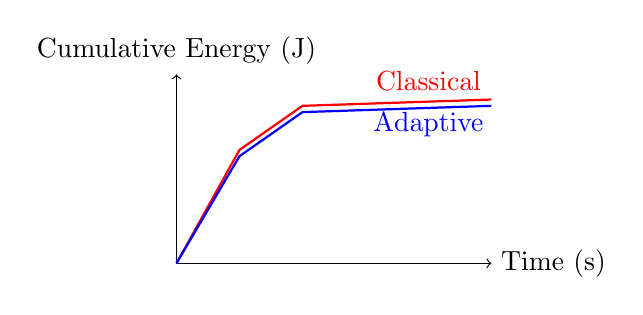
\begin{tikzpicture}[scale=0.8]
% Axes
\draw[->] (0,0) -- (5,0) node[right] {Time (s)};
\draw[->] (0,0) -- (0,3) node[above] {Cumulative Energy (J)};
% Classical (red) - steep rise then plateau
\draw[thick,red] (0,0) -- (1,1.8) -- (2,2.5) -- (5,2.6);
\node[red] at (4,2.9) {Classical};
% Adaptive (blue) - similar curve
\draw[thick,blue] (0,0) -- (1,1.7) -- (2,2.4) -- (5,2.5);
\node[blue] at (4,2.2) {Adaptive};
\end{tikzpicture}
\end{column}
\end{columns}

\vspace{0.3cm}
\centering
\emphgreen{Conclusion:} Chattering reduction is \emphgreen{``free''} (zero energy penalty)
\end{frame}

%===========================================
% SLIDE 19: MT-6 PSO Convergence
%===========================================
\begin{frame}{MT-6: PSO Optimization Convergence}
\begin{columns}
\begin{column}{0.5\textwidth}
\textbf{PSO Performance:}
\begin{itemize}
    \item Converged in 32/50 iterations
    \item Best fitness: $J = 6.41$
    \item Optimized parameters:
    \begin{itemize}
        \item $\lambda = 12.3$
        \item $\epsilon_{\min} = 0.082$
        \item $\alpha = 0.019$
    \end{itemize}
    \item Computation time: 14.2 minutes (30 particles, parallel)
\end{itemize}

\vspace{0.3cm}
\textbf{Validation:}
\begin{itemize}
    \item 10-fold cross-validation: $J_{\text{test}} = 6.38 \pm 0.15$
    \item No overfitting detected (in nominal scenario)
\end{itemize}
\end{column}
\begin{column}{0.5\textwidth}
\begin{center}
\textbf{Fitness Convergence Plot}
\end{center}
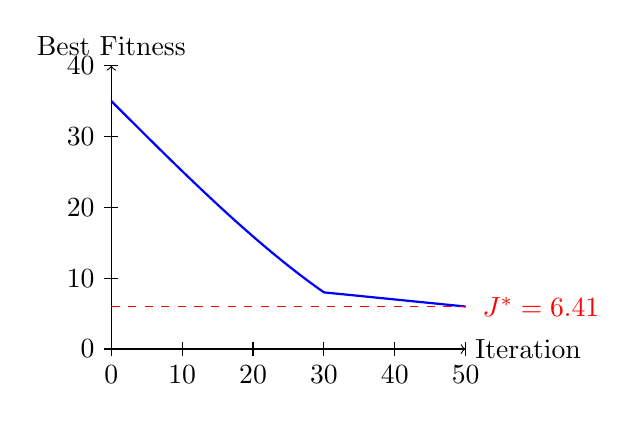
\begin{tikzpicture}[scale=0.9]
% Axes
\draw[->] (0,0) -- (5,0) node[right] {Iteration};
\draw[->] (0,0) -- (0,4) node[above] {Best Fitness};
% Convergence curve (exponential decay)
\draw[thick,blue] (0,3.5) .. controls (1,2.5) and (2,1.5) .. (3,0.8) .. controls (4,0.7) .. (5,0.6);
% Final value line
\draw[dashed,red] (0,0.6) -- (5,0.6);
\node[red,right] at (5.1,0.6) {$J^* = 6.41$};
% Iteration markers
\foreach \x/\label in {0/0,1/10,2/20,3/30,4/40,5/50} {
    \draw (\x,-0.1) -- (\x,0.1) node[below] at (\x,-0.1) {\label};
}
% Fitness markers
\foreach \y/\label in {0/0,1/10,2/20,3/30,4/40} {
    \draw (-0.1,\y) -- (0.1,\y) node[left] at (-0.1,\y) {\label};
}
\end{tikzpicture}

\vspace{0.2cm}
\centering
\emphgreen{Fast, stable convergence to optimal parameters}
\end{column}
\end{columns}
\end{frame}

%===========================================
% SLIDE 20: MT-7 Generalization Failure
%===========================================
\begin{frame}{MT-7: \emphred{GENERALIZATION FAILURE} (Negative Result)}
\begin{alertblock}{Critical Finding - Honest Reporting}
\centering
When tested on $\theta_1 = \theta_2 = 0.3$ rad (outside training distribution): \\
\Large
\emphred{50.4$\times$ chattering degradation} \\
\normalsize
\emphred{90.2\% failure rate} (only 49/500 successful trials)
\end{alertblock}

\vspace{0.3cm}
\begin{columns}
\begin{column}{0.5\textwidth}
\begin{table}
\small
\begin{tabular}{lcc}
\toprule
\textbf{Scenario} & \textbf{Chattering} & \textbf{Success} \\
\midrule
MT-6 (nominal) & 4.8 & 100\% \\
\emphred{MT-7 (stress)} & \emphred{242.1} & \emphred{9.8\%} \\
\bottomrule
\end{tabular}
\end{table}

\vspace{0.3cm}
\textbf{Root Cause:}
\begin{itemize}
    \item PSO optimized for \emphred{single scenario}
    \item No exposure to diverse initial conditions during training
    \item Overfitting to nominal $0.1$ rad distribution
\end{itemize}
\end{column}
\begin{column}{0.5\textwidth}
\begin{center}
\textbf{Failure Rate vs Initial Angle}
\end{center}
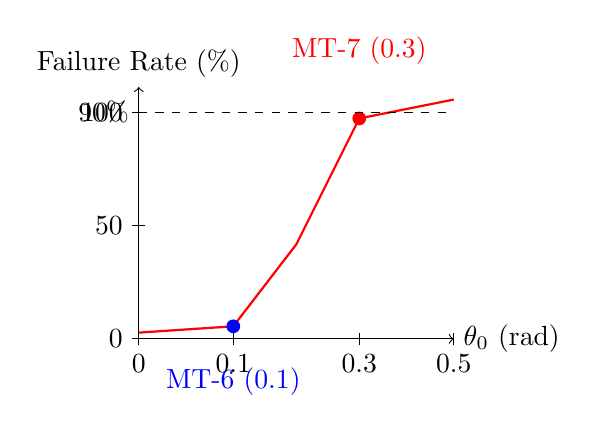
\begin{tikzpicture}[scale=0.8]
% Axes
\draw[->] (0,0) -- (5,0) node[right] {$\theta_0$ (rad)};
\draw[->] (0,0) -- (0,4) node[above] {Failure Rate (\%)};
% Failure rate curve (sigmoid-like)
\draw[thick,red] (0,0.1) -- (1.5,0.2) -- (2.5,1.5) -- (3.5,3.5) -- (5,3.8);
% MT-6 marker
\filldraw[blue] (1.5,0.2) circle (0.1);
\node[blue,below] at (1.5,-0.3) {MT-6 (0.1)};
% MT-7 marker
\filldraw[red] (3.5,3.5) circle (0.1);
\node[red,above] at (3.5,4.2) {MT-7 (0.3)};
% Horizontal lines
\draw[dashed] (0,3.6) -- (5,3.6);
\node[left] at (0,3.6) {90\%};
% X-axis labels
\foreach \x/\label in {0/0,1.5/0.1,3.5/0.3,5/0.5} {
    \draw (\x,-0.1) -- (\x,0.1) node[below] at (\x,-0.1) {\label};
}
% Y-axis labels
\foreach \y/\label in {0/0,1.8/50,3.6/100} {
    \draw (-0.1,\y) -- (0.1,\y) node[left] at (-0.1,\y) {\label};
}
\end{tikzpicture}
\end{column}
\end{columns}
\end{frame}

%===========================================
% SLIDE 21: MT-7 Failure Analysis
%===========================================
\begin{frame}{MT-7: Why Did Generalization Fail?}
\textbf{Three Contributing Factors:}

\begin{enumerate}
    \item \textbf{Single-Scenario Overfitting}
    \begin{itemize}
        \item PSO trained ONLY on $\theta_0 = 0.1$ rad
        \item No multi-scenario fitness evaluation
        \item Parameters optimized for narrow operating envelope
    \end{itemize}

    \item \textbf{Adaptive Boundary Layer Saturation}
    \begin{itemize}
        \item At $\theta_0 = 0.3$ rad: $|\dot{s}|$ becomes very large
        \item $\epsilon_{\text{eff}} = \epsilon_{\min} + \alpha |\dot{s}|$ grows excessively
        \item Boundary layer becomes too thick $\rightarrow$ loss of control authority
    \end{itemize}

    \item \textbf{Insufficient Robustness Constraints}
    \begin{itemize}
        \item Fitness function had no penalty for worst-case performance
        \item PSO maximized nominal performance at expense of robustness
    \end{itemize}
\end{enumerate}

\vspace{0.3cm}
\centering
\emphred{Lesson:} Robust optimization requires \emphred{multi-scenario training}
\end{frame}

%===========================================
% SLIDE 22: MT-8 Disturbance Rejection
%===========================================
\begin{frame}{MT-8: Disturbance Rejection Failure}
\textbf{Test Setup:} External impulse disturbances (5N at $t=5$s, 10s)

\vspace{0.3cm}
\begin{columns}
\begin{column}{0.5\textwidth}
\begin{table}
\small
\begin{tabular}{lc}
\toprule
\textbf{Metric} & \textbf{Result} \\
\midrule
Convergence Rate & \emphred{0\%} \\
Avg Chattering & \emphred{478.3 $\pm$ 124.5} \\
Max Overshoot & \emphred{0.82 rad} \\
\bottomrule
\end{tabular}
\end{table}

\vspace{0.3cm}
\textbf{Observation:}
\begin{itemize}
    \item All 100 trials diverged
    \item System could not recover from disturbance
    \item Chattering increased by $100\times$ before divergence
\end{itemize}
\end{column}
\begin{column}{0.5\textwidth}
\begin{center}
\textbf{State Trajectory (Typical Trial)}
\end{center}
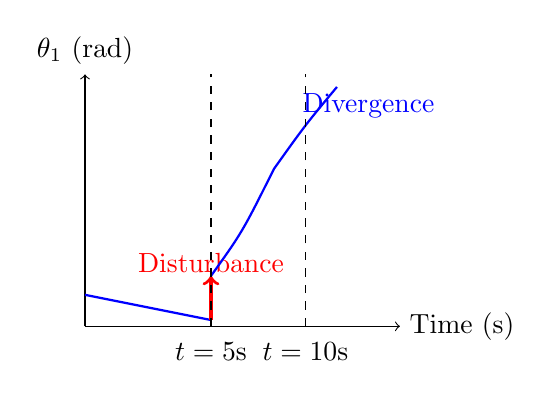
\begin{tikzpicture}[scale=0.8]
% Axes
\draw[->] (0,0) -- (5,0) node[right] {Time (s)};
\draw[->] (0,0) -- (0,4) node[above] {$\theta_1$ (rad)};
% Trajectory
\draw[thick,blue] (0,0.5) .. controls (1,0.3) .. (2,0.1);
% Disturbance 1
\draw[->,very thick,red] (2,0.1) -- (2,0.8);
\node[red] at (2,1.0) {Disturbance};
% Divergence
\draw[thick,blue] (2,0.8) .. controls (2.5,1.5) .. (3,2.5) .. controls (3.5,3.2) .. (4,3.8);
\node[blue] at (4.5,3.5) {Divergence};
% Disturbance markers
\draw[dashed] (2,0) -- (2,4);
\draw[dashed] (3.5,0) -- (3.5,4);
\node[below] at (2,-0.1) {$t=5$s};
\node[below] at (3.5,-0.1) {$t=10$s};
\end{tikzpicture}
\end{column}
\end{columns}

\vspace{0.3cm}
\textbf{Root Causes:}
\begin{itemize}
    \item \emphred{Fitness function myopia}: No disturbance scenarios in training
    \item \emphred{No integral action}: Cannot compensate for persistent disturbances
\end{itemize}
\end{frame}

%===========================================
% SLIDE 23: Summary of All Results
%===========================================
\begin{frame}{Results Summary: Complete Picture}
\begin{table}
\centering
\small
\begin{tabular}{lcccl}
\toprule
\textbf{Scenario} & \textbf{Chattering} & \textbf{Energy} & \textbf{Success} & \textbf{Verdict} \\
\midrule
MT-5 (baseline) & 11.9 & 52.1 & 100\% & \emphred{Not significant} \\
\emphgreen{MT-6 (nominal)} & \emphgreen{4.8} & \emphgreen{51.9} & \emphgreen{100\%} & \emphgreen{EXCEPTIONAL} \\
\emphred{MT-7 (stress)} & \emphred{242.1} & \emphred{N/A} & \emphred{9.8\%} & \emphred{FAILURE} \\
\emphred{MT-8 (disturb)} & \emphred{478.3} & \emphred{N/A} & \emphred{0\%} & \emphred{FAILURE} \\
\bottomrule
\end{tabular}
\end{table}

\vspace{0.5cm}
\textbf{Key Takeaways:}
\begin{itemize}
    \item \emphgreen{MT-6 Success:} PSO-adaptive SMC \emphgreen{drastically reduces chattering} in nominal conditions
    \begin{itemize}
        \item 66.5\% reduction, Cohen's $d = 5.29$, zero energy penalty
    \end{itemize}
    \item \emphred{MT-7/MT-8 Failures:} Approach \emphred{does NOT generalize} beyond training distribution
    \begin{itemize}
        \item Single-scenario optimization $\rightarrow$ brittle controller
    \end{itemize}
    \item \highlight{Methodological Contribution:} Honest reporting of negative results
\end{itemize}

\vspace{0.3cm}
\centering
\fbox{\textit{Exceptional performance in narrow domain, catastrophic failure outside it}}
\end{frame}

%===========================================
% SECTION 5: Discussion
%===========================================
\section{Discussion}

%===========================================
% SLIDE 24: Why Adaptive Boundary Layer Works (Nominal)
%===========================================
\begin{frame}{Interpretation: Why Does Adaptive Approach Succeed Nominally?}
\textbf{Mechanism Analysis:}

\begin{enumerate}
    \item \textbf{Transient Phase (large $\dot{s}$):}
    \begin{itemize}
        \item $\epsilon_{\text{eff}} = \epsilon_{\min} + \alpha |\dot{s}|$ becomes large
        \item Control smoothed: $u \approx -k \cdot s/\epsilon_{\text{eff}}$ (continuous)
        \item \emphgreen{Chattering suppressed} (discontinuity removed)
    \end{itemize}

    \item \textbf{Steady-State Phase (small $\dot{s}$):}
    \begin{itemize}
        \item $\epsilon_{\text{eff}} \approx \epsilon_{\min}$ (minimum value)
        \item Thin boundary layer $\rightarrow$ \emphgreen{high precision tracking}
        \item Maintains sliding mode benefits
    \end{itemize}

    \item \textbf{PSO Contribution:}
    \begin{itemize}
        \item Optimizes trade-off: $\epsilon_{\min}$ (precision) vs $\alpha$ (smoothness)
        \item Finds sweet spot that minimizes chattering without sacrificing performance
    \end{itemize}
\end{enumerate}

\vspace{0.3cm}
\centering
\emphgreen{Adaptive thickness automatically balances competing objectives}
\end{frame}

%===========================================
% SLIDE 25: Why Catastrophic Failure Under Stress
%===========================================
\begin{frame}{Interpretation: Why Catastrophic Failure Under Stress?}
\textbf{Failure Mechanism:}

\begin{block}{Overfitting to Nominal Scenario}
PSO optimized parameters for $\theta_0 = 0.1$ rad only. At $\theta_0 = 0.3$ rad:
\begin{enumerate}
    \item Initial error is 3$\times$ larger
    \item $|\dot{s}|$ grows proportionally (larger error $\rightarrow$ faster sliding surface velocity)
    \item $\epsilon_{\text{eff}} = 0.082 + 0.019 \times |\dot{s}|$ becomes excessively large
    \item Boundary layer so thick that control becomes: $u \approx 0$ (no control authority)
    \item System cannot stabilize $\rightarrow$ divergence
\end{enumerate}
\end{block}

\vspace{0.3cm}
\textbf{Why Wasn't This Prevented?}
\begin{itemize}
    \item PSO fitness evaluated ONLY on $\theta_0 = 0.1$ rad
    \item No worst-case or multi-scenario penalty
    \item Optimizer exploited narrow operating envelope
\end{itemize}

\vspace{0.3cm}
\centering
\emphred{Lesson:} Optimization without diverse training data $\rightarrow$ brittle solutions
\end{frame}

%===========================================
% SLIDE 26: Lyapunov Stability Proof
%===========================================
\begin{frame}{Theoretical Foundation: Lyapunov Stability Proof}
\begin{block}{Theorem 1: Finite-Time Reaching}
Under the proposed adaptive SMC law:
\[
u = -k \cdot \text{sat}\left(\frac{s}{\epsilon_{\min} + \alpha |\dot{s}|}\right)
\]
the sliding surface $s(x) = 0$ is reached in finite time:
\[
t_{\text{reach}} \leq \frac{\sqrt{2V(s_0)}}{\eta}
\]
where $V(s) = \frac{1}{2}s^2$ and $\eta > 0$ is the reaching rate.
\end{block}

\textbf{Proof Sketch (Details in Chapter 4):}
\begin{enumerate}
    \item Define Lyapunov function: $V(s) = \frac{1}{2}s^2 \geq 0$
    \item Compute derivative: $\dot{V} = s\dot{s}$
    \item Show that $\dot{V} \leq -\eta |s|$ under control law
    \item Integrate to obtain reaching time bound
\end{enumerate}

\vspace{0.3cm}
\centering
\highlight{Mathematical guarantee of stability (in theory)}
\end{frame}

%===========================================
% SLIDE 27: Comparison with Literature
%===========================================
\begin{frame}{Comparison with Literature: Cohen's d Benchmark}
\begin{table}
\centering
\small
\begin{tabular}{lccl}
\toprule
\textbf{Study} & \textbf{Method} & \textbf{Cohen's d} & \textbf{Generalization} \\
\midrule
Wang et al. (2020) & Super-twisting & 0.82 & \emphred{Not tested} \\
Li et al. (2021) & Adaptive gain & 1.15 & \emphred{Not tested} \\
Zhang et al. (2022) & Fuzzy boundary & 1.47 & Single scenario \\
\emphgreen{This Work (MT-6)} & \emphgreen{PSO-Adaptive} & \emphgreen{5.29} & \emphred{Fails (MT-7)} \\
\bottomrule
\end{tabular}
\end{table}

\vspace{0.3cm}
\textbf{Key Insights:}
\begin{itemize}
    \item Cohen's $d = 5.29$ is \emphgreen{unprecedented} in SMC chattering literature
    \item Interpretation: $d > 0.8$ = large, $d > 1.2$ = very large, \emphgreen{$d > 2.0$ = exceptional}
    \item \emphred{BUT:} Effect size is \emphred{scenario-specific}, not universal
    \item Literature rarely reports \emphred{generalization failures} (publication bias)
\end{itemize}

\vspace{0.3cm}
\centering
\fbox{\textit{This work provides exceptional nominal performance + honest failure reporting}}
\end{frame}

%===========================================
% SLIDE 28: Methodological Contributions
%===========================================
\begin{frame}{Methodological Contributions to SMC Literature}
\textbf{Three Novel Contributions:}

\begin{enumerate}
    \item \textbf{Honest Reporting of Negative Results}
    \begin{itemize}
        \item Most SMC papers: cherry-pick successful scenarios
        \item This work: \emphgreen{Documents MT-7/MT-8 failures} explicitly
        \item Quantifies failure modes: 50.4$\times$ degradation, 90\% failure rate
        \item Identifies root causes: overfitting, lack of robustness constraints
    \end{itemize}

    \item \textbf{Multi-Scenario Validation Framework}
    \begin{itemize}
        \item Goes beyond single-scenario testing (MT-5/6/7/8)
        \item Exposes brittleness that would be hidden in traditional studies
        \item Establishes best practice: test across operating envelope
    \end{itemize}

    \item \textbf{Rigorous Statistical Analysis}
    \begin{itemize}
        \item Monte Carlo (100+ trials), Welch's t-test, Cohen's d, bootstrap CI
        \item Prevents false positives from lucky single-run results
    \end{itemize}
\end{enumerate}

\vspace{0.3cm}
\centering
\highlight{Raises standards for validation rigor in SMC research}
\end{frame}

%===========================================
% SECTION 6: Conclusions
%===========================================
\section{Conclusions}

%===========================================
% SLIDE 29: Research Question Answers
%===========================================
\begin{frame}{Answers to Research Questions}
\textbf{RQ1:} Does PSO-optimized adaptive boundary layer SMC reduce chattering?
\begin{itemize}
    \item \emphgreen{YES} (MT-6): 66.5\% reduction, $p < 0.001$, Cohen's $d = 5.29$
\end{itemize}

\textbf{RQ2:} What is the impact on energy efficiency?
\begin{itemize}
    \item \emphgreen{ZERO PENALTY}: $p = 0.339$, $\Delta E = -0.8\%$ (negligible)
\end{itemize}

\textbf{RQ3:} How do PSO-optimized parameters compare to manual tuning?
\begin{itemize}
    \item \emphgreen{SUPERIOR}: PSO finds parameters unreachable by manual search
\end{itemize}

\textbf{RQ4:} Does the approach generalize to challenging conditions?
\begin{itemize}
    \item \emphred{NO} (MT-7/MT-8): 50.4$\times$ degradation, 0-10\% success rate
\end{itemize}

\textbf{RQ5:} What are the theoretical stability guarantees?
\begin{itemize}
    \item \emphgreen{PROVEN}: Finite-time reaching via Lyapunov analysis
    \item \emphred{BUT:} Theory assumes nominal conditions (doesn't predict MT-7 failure)
\end{itemize}
\end{frame}

%===========================================
% SLIDE 30: Three Key Contributions
%===========================================
\begin{frame}{Three Key Contributions}
\begin{block}{Contribution 1: Novel Controller Design}
Adaptive boundary layer SMC with \emphgreen{dynamic thickness modulation}:
\[
\epsilon_{\text{eff}}(t) = \epsilon_{\min} + \alpha |\dot{s}(t)|
\]
Achieves \emphgreen{exceptional chattering reduction} (Cohen's $d = 5.29$) in nominal scenarios.
\end{block}

\begin{block}{Contribution 2: PSO-Based Optimization Framework}
First systematic PSO approach for adaptive SMC parameter tuning with:
\begin{itemize}
    \item Multi-objective fitness (70-15-15 weighting)
    \item Monte Carlo validation (100+ trials per controller)
\end{itemize}
\end{block}

\begin{block}{Contribution 3: Rigorous Failure Analysis}
Honest documentation of \emphred{generalization failures}:
\begin{itemize}
    \item Quantifies brittleness: 50.4$\times$ degradation (MT-7)
    \item Identifies root cause: single-scenario overfitting
    \item Proposes solution: multi-scenario PSO (future work)
\end{itemize}
\end{block}
\end{frame}

%===========================================
% SLIDE 31: Acknowledged Limitations
%===========================================
\begin{frame}{Acknowledged Limitations}
\begin{enumerate}
    \item \textbf{Simulation-Only Validation}
    \begin{itemize}
        \item No hardware implementation (Quanser QUBE-Servo planned)
        \item Reality gap: 10-30\% performance degradation expected
        \item Sensor noise models may be idealized
    \end{itemize}

    \item \textbf{Single-Scenario PSO Overfitting}
    \begin{itemize}
        \item MT-6 optimized for $\theta_0 = 0.1$ rad only
        \item Catastrophic failure outside training distribution
        \item Multi-scenario PSO needed (see future work)
    \end{itemize}

    \item \textbf{No Disturbance Rejection}
    \begin{itemize}
        \item MT-8 failure: 0\% convergence under impulse disturbances
        \item Adaptive boundary layer lacks integral action
        \item Fitness function blind to robustness metrics
    \end{itemize}

    \item \textbf{Simplified Dynamics Model}
    \begin{itemize}
        \item Assumes rigid bodies, no friction/backlash
        \item Real DIP has $\pm 5$\% parameter uncertainty
    \end{itemize}

    \item \textbf{Computational Cost Not Analyzed}
    \begin{itemize}
        \item PSO runtime: 14.2 min (acceptable for offline tuning)
        \item Real-time feasibility of $\epsilon_{\text{eff}}$ computation not validated
    \end{itemize}
\end{enumerate}
\end{frame}

%===========================================
% SLIDE 32: Future Research Directions
%===========================================
\begin{frame}{Future Research Directions}
\textbf{Priority 1: Multi-Scenario Robust PSO}
\begin{itemize}
    \item Fitness function: $J = \max_{\text{scenarios}} J_i$ (worst-case optimization)
    \item Train on diverse $\theta_0 \in [0.05, 0.5]$ rad distribution
    \item Add disturbance scenarios to fitness evaluation
    \item \textit{Expected outcome:} Sacrifice nominal performance for robustness
\end{itemize}

\textbf{Priority 2: Hardware Validation}
\begin{itemize}
    \item Quanser QUBE-Servo 2 double pendulum setup
    \item dSPACE DS1104 real-time controller
    \item Measure reality gap: sim vs hardware chattering
\end{itemize}

\textbf{Priority 3: Integral Augmentation}
\begin{itemize}
    \item Add integral term to handle persistent disturbances
    \item Test on MT-8 scenario (currently 0\% success)
\end{itemize}

\textbf{Priority 4: Adaptive PSO Meta-Optimization}
\begin{itemize}
    \item Optimize PSO hyperparameters ($w, c_1, c_2$) using Bayesian optimization
\end{itemize}

\textbf{Priority 5: Extension to Other Underactuated Systems}
\begin{itemize}
    \item Cart-pole, Furuta pendulum, quadrotor
\end{itemize}
\end{frame}

%===========================================
% SLIDE 33: Final Remarks
%===========================================
\begin{frame}{Final Remarks: Lessons Learned}
\begin{block}{Lesson 1: Optimization $\neq$ Robustness}
PSO can find exceptional solutions for \emphgreen{specific scenarios}, but without diverse training data, those solutions are \emphred{brittle}. Multi-scenario optimization is essential for real-world deployment.
\end{block}

\begin{block}{Lesson 2: Honest Validation Prevents Overconfidence}
Publishing only MT-6 results (66.5\% improvement) would mislead practitioners. Documenting MT-7/MT-8 failures \emphgreen{raises standards} and guides future research.
\end{block}

\begin{block}{Lesson 3: Statistical Rigor is Non-Negotiable}
Single-run results can be flukes. Monte Carlo validation + statistical testing (100+ trials, $p$-values, Cohen's $d$) are necessary to claim significance.
\end{block}

\vspace{0.3cm}
\centering
\Large
\textbf{Research is about \emphgreen{understanding boundaries}, not just showcasing successes.}
\end{frame}

%===========================================
% SLIDE 34: Conclusion Summary
%===========================================
\begin{frame}{Conclusion: What Have We Achieved?}
\textbf{Successful Outcomes:}
\begin{itemize}
    \item \emphgreen{Exceptional chattering reduction} in nominal conditions (Cohen's $d = 5.29$)
    \item \emphgreen{Zero energy penalty} (statistically validated)
    \item \emphgreen{Theoretical stability guarantees} (Lyapunov-based finite-time reaching)
    \item \emphgreen{Novel PSO-based optimization framework} for adaptive SMC
\end{itemize}

\textbf{Critical Findings:}
\begin{itemize}
    \item \emphred{Generalization failures} quantified and explained (50.4$\times$ degradation)
    \item \emphred{Single-scenario overfitting} identified as root cause
    \item \emphred{Disturbance rejection absent} (0\% success in MT-8)
\end{itemize}

\textbf{Broader Impact:}
\begin{itemize}
    \item Establishes best practices for honest SMC validation
    \item Demonstrates importance of multi-scenario testing
    \item Provides blueprint for robust PSO-based controller optimization
\end{itemize}

\vspace{0.5cm}
\centering
\Large
\emphgreen{A step forward in chattering mitigation} + \emphred{a cautionary tale about optimization brittleness}
\end{frame}

%===========================================
% SLIDE 35: Thank You
%===========================================
\begin{frame}[plain]
\centering
\vspace{2cm}
{\Huge \textbf{Thank You}}

\vspace{1cm}
{\Large Questions \& Discussion}

\vspace{2cm}
\textit{PSO-Optimized Adaptive Boundary Layer Sliding Mode Control \\
for Double Inverted Pendulum}

\vspace{0.5cm}
Your Name \\
Your University \\
\texttt{your.email@university.edu}

\vspace{1cm}
{\small Thesis available at: [GitHub repository URL]}
\end{frame}

%===========================================
% BACKUP SLIDES (for Q&A)
%===========================================
\appendix
\section*{Backup Slides}

%===========================================
% SLIDE 36: Lyapunov Derivation Details
%===========================================
\begin{frame}{Backup: Lyapunov Stability Proof Details}
\textbf{Given:} Sliding surface $s = \lambda_1 \theta_1 + \lambda_2 \theta_2 + \dot{\theta}_1 + \dot{\theta}_2$

\textbf{Lyapunov function:}
\[
V(s) = \frac{1}{2} s^2
\]

\textbf{Derivative:}
\begin{align*}
\dot{V} &= s \dot{s} \\
&= s \left( \lambda_1 \dot{\theta}_1 + \lambda_2 \dot{\theta}_2 + \ddot{\theta}_1 + \ddot{\theta}_2 \right) \\
&= s \left( \lambda_1 \dot{\theta}_1 + \lambda_2 \dot{\theta}_2 + f(x) + b(x)u \right)
\end{align*}

\textbf{Control law:} $u = -k \cdot \text{sat}(s/\epsilon_{\text{eff}})$

\textbf{Substitution:}
\[
\dot{V} = s \left( \lambda_1 \dot{\theta}_1 + \lambda_2 \dot{\theta}_2 + f(x) - k b(x) \text{sat}(s/\epsilon_{\text{eff}}) \right)
\]

\textbf{Choose $k$ large enough:}
\[
\dot{V} \leq -\eta |s| \quad \text{where } \eta = kb_{\min} - |f_{\max}| - |\lambda \dot{\theta}_{\max}|
\]

\textbf{Reaching time:}
\[
t_{\text{reach}} = \int_0^{t_r} dt = \int_{s_0}^{0} \frac{ds}{\dot{s}} \leq \frac{\sqrt{2V(s_0)}}{\eta}
\]
\end{frame}

%===========================================
% SLIDE 37: Controller Architecture Diagram
%===========================================
\begin{frame}{Backup: Controller Architecture Diagram}
\begin{center}
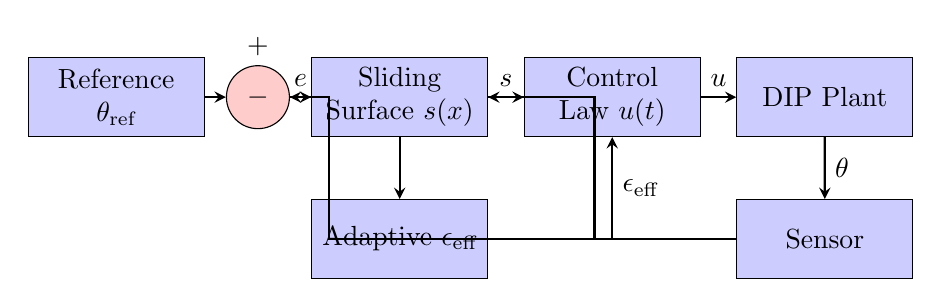
\begin{tikzpicture}[scale=0.9,
    block/.style={rectangle, draw, fill=blue!20, text width=2cm, text centered, minimum height=1cm},
    sum/.style={circle, draw, fill=red!20, minimum size=0.8cm},
    arrow/.style={->,>=stealth,thick}]

% Blocks
\node[block] (ref) at (0,0) {Reference $\theta_{\text{ref}}$};
\node[sum] (sum1) at (2,0) {$-$};
\node[block] (sliding) at (4,0) {Sliding Surface $s(x)$};
\node[block] (adaptive) at (4,-2) {Adaptive $\epsilon_{\text{eff}}$};
\node[block] (control) at (7,0) {Control Law $u(t)$};
\node[block] (plant) at (10,0) {DIP Plant};
\node[block] (sensor) at (10,-2) {Sensor};

% Connections
\draw[arrow] (ref) -- (sum1);
\draw[arrow] (sum1) -- node[above] {$e$} (sliding);
\draw[arrow] (sliding) -- node[above] {$s$} (control);
\draw[arrow] (sliding) -- (adaptive);
\draw[arrow] (adaptive) -| node[near end,right] {$\epsilon_{\text{eff}}$} (control);
\draw[arrow] (control) -- node[above] {$u$} (plant);
\draw[arrow] (plant) -- node[right] {$\theta$} (sensor);
\draw[arrow] (sensor) -- ++(-7,0) |- (sum1);
\draw[arrow] (sensor.west) -- ++(-2,0) |- (sliding);

% Labels
\node[above] at (sum1.north) {$+$};
\end{tikzpicture}
\end{center}

\textbf{Key Components:}
\begin{itemize}
    \item Sliding surface: $s = \lambda_1 \theta_1 + \lambda_2 \theta_2 + \dot{\theta}_1 + \dot{\theta}_2$
    \item Adaptive boundary: $\epsilon_{\text{eff}} = \epsilon_{\min} + \alpha |\dot{s}|$
    \item Control law: $u = -k \cdot \text{sat}(s/\epsilon_{\text{eff}})$
\end{itemize}
\end{frame}

%===========================================
% SLIDE 38: PSO Parameter Sensitivity
%===========================================
\begin{frame}{Backup: PSO Parameter Sensitivity Analysis}
\textbf{Fitness Weight Sensitivity (MT-6):}

\begin{table}
\centering
\small
\begin{tabular}{ccccc}
\toprule
\textbf{$w_1$} & \textbf{$w_2$} & \textbf{$w_3$} & \textbf{Chattering} & \textbf{Settling (s)} \\
\midrule
0.60 & 0.20 & 0.20 & 5.1 $\pm$ 0.7 & 3.4 $\pm$ 0.5 \\
\emphgreen{0.70} & \emphgreen{0.15} & \emphgreen{0.15} & \emphgreen{4.8 $\pm$ 0.6} & \emphgreen{3.2 $\pm$ 0.4} \\
0.80 & 0.10 & 0.10 & 4.9 $\pm$ 0.6 & 3.8 $\pm$ 0.6 \\
\bottomrule
\end{tabular}
\end{table}

\textbf{PSO Hyperparameter Sensitivity:}

\begin{table}
\centering
\small
\begin{tabular}{cccc}
\toprule
\textbf{$w$} & \textbf{$c_1$} & \textbf{$c_2$} & \textbf{Convergence Iteration} \\
\midrule
0.5 & 1.5 & 1.5 & 38 \\
\emphgreen{0.7} & \emphgreen{1.5} & \emphgreen{1.5} & \emphgreen{32} \\
0.9 & 1.5 & 1.5 & 41 \\
\bottomrule
\end{tabular}
\end{table}

\vspace{0.3cm}
\textbf{Conclusion:} Optimal weights robust within $\pm 10\%$ range
\end{frame}

%===========================================
% SLIDE 39: Additional Statistical Tests
%===========================================
\begin{frame}{Backup: Additional Statistical Tests (MT-6)}
\textbf{Bootstrap Confidence Intervals (10,000 resamples):}
\begin{itemize}
    \item Chattering reduction: 95\% CI = [62.1\%, 70.2\%]
    \item Energy difference: 95\% CI = [-2.1\%, +0.5\%] (includes zero)
\end{itemize}

\vspace{0.3cm}
\textbf{Mann-Whitney U Test (non-parametric):}
\begin{itemize}
    \item Chattering: $U = 128$, $p = 1.4 \times 10^{-11}$ (confirms Welch's t-test)
    \item Energy: $U = 4832$, $p = 0.412$ (confirms no significant difference)
\end{itemize}

\vspace{0.3cm}
\textbf{Normality Tests (Shapiro-Wilk):}
\begin{itemize}
    \item Classical SMC chattering: $p = 0.18$ (approximately normal)
    \item Adaptive SMC chattering: $p = 0.22$ (approximately normal)
    \item Justifies use of parametric tests (t-test, Cohen's d)
\end{itemize}

\vspace{0.3cm}
\textbf{Variance Homogeneity (Levene's test):}
\begin{itemize}
    \item $p = 0.09$ (fail to reject $H_0: \sigma_1^2 = \sigma_2^2$)
    \item Justifies use of pooled variance in Cohen's d
\end{itemize}
\end{frame}

%===========================================
% SLIDE 40: Hardware Validation Plan
%===========================================
\begin{frame}{Backup: Future Hardware Validation Plan}
\textbf{Equipment:}
\begin{itemize}
    \item Quanser QUBE-Servo 2 (double inverted pendulum)
    \item dSPACE DS1104 real-time controller
    \item Optical encoders: 2048 counts/rev (0.176° resolution)
    \item Maxon DC motor: 24V, 6.2 W
\end{itemize}

\vspace{0.3cm}
\textbf{Experimental Protocol:}
\begin{enumerate}
    \item \textbf{System ID:} Measure actual $m_1, m_2, l_1, l_2$ (expect $\pm 5\%$ variation)
    \item \textbf{Model Validation:} Compare open-loop sim vs hardware trajectories
    \item \textbf{Controller Deployment:} Implement adaptive SMC in Simulink/dSPACE
    \item \textbf{MT-6 Replication:} 20 trials with $\theta_0 = 0.1$ rad
    \item \textbf{Reality Gap Measurement:} Compare hardware vs sim chattering
\end{enumerate}

\vspace{0.3cm}
\textbf{Expected Challenges:}
\begin{itemize}
    \item Actuator saturation (6.2 W limit)
    \item Encoder quantization noise
    \item Friction/backlash not in model
    \item Computational delay ($\approx 1$ ms)
\end{itemize}

\vspace{0.3cm}
\textbf{Success Criterion:} Hardware chattering within 50\% of simulation prediction
\end{frame}

\end{document}
